\documentclass[a4paper, 11pt, final, garamond]{book}
\usepackage{cours-preambule}

\makeatletter
\renewcommand{\@chapapp}{Devoir surveill\'e -- num\'ero}
\makeatother

\begin{document}
\setcounter{chapter}{0}

\def\lspace{25}

\chapter{Commentaires sur le DS n\degree01}
\section{Commentaires généraux}

\subsection{Présentation}

\begin{itemize}
	\item Globalement TB sur la présentation, mais il y a quand même 33 points de
	      malus cumulés.
	\item Attention à la numérotation des copies~: en bas à droite, et il faut
	      indiquer le \textbf{nombre total de copies}, sinon c'est inutile.
	\item Encadrez littéral, soulignez numérique.
	\item Cadre pour mes remarques plus grand, j'écris parfois beaucoup.
	\item Préliminaire va dans remarques antérieures.
	\item Pas mal sur les commentaires antérieurs, mais ne déformez pas mes propos
	      s'il vous plaît. Ils sont mesurés et respectent ma posture en tant
	      qu'enseignante. Par exemple, e n'ai jamais dit «~Soyez intelligent~» et je
	      ne le ferai jamais, ça serait supposer que vous ne l'êtes pas, et c'est
	      faux. Total de 60 points bonus.
	\item N'oubliez pas le cadre remarques personnelles, à compléter pendant le DS
	      et une fois que je vous ai rendu votre copie en reprenant vos erreurs. Utile
	      à la fin de l'année et l'année prochaine pendant vos révisions.
	\item \textbf{Ne pas rendre l'annexe si pas complétée}.
	\item \xul{Pas besoin de mettre un cadre sur chaque copie}.
	\item Indiquer «~\textbf{Voir annexe}~» quand vous complétez l'annexe~!
	\item Indiquer clairement quand vous reprenez une question ou un problème plus
	      tard, à l'aide d'une astérisque et du numéro de page/copie si pertinent.
	      \xul{Sinon je ne lirai pas}.
\end{itemize}

\subsection{Sur l'optique}
\begin{itemize}
	\item Pas besoin de démontrer les formules du grandissement~! Mais c'est super
	      et nécessaire de \textbf{savoir} le faire au cas où vous l'oubliez.
	\item Les exercices étant indépendants, \textbf{vous ne pouvez pas invoquer un
		      résultat ou une démonstration d'un autre exercice}. Notamment, il
	      \textbf{faut} réécrire la relation de conjugaison dans chaque nouvel
	      exercice et ne pas catapulter les résultats de l'exercice 1 par exemple.
	\item Trop de résultats faux basés sur des «~(lentille divergente)~», alors
	      que \textbf{rien} ne justifie un traitement différent.
\end{itemize}

\begin{tcn}[bld,cnt,fontupper=\Large](impo){Rappel important}
	Les lentilles divergentes n'ont \textit{rien} de spécial~!
\end{tcn}

Si vous justifiez un résultat par «~car $\Lc$ est divergente~», alors c'est
faux. Seule exception~: dire $f' < 0$ (car $\Lc$ est divergente).

\begin{figure}[htbp!]
	\centering
	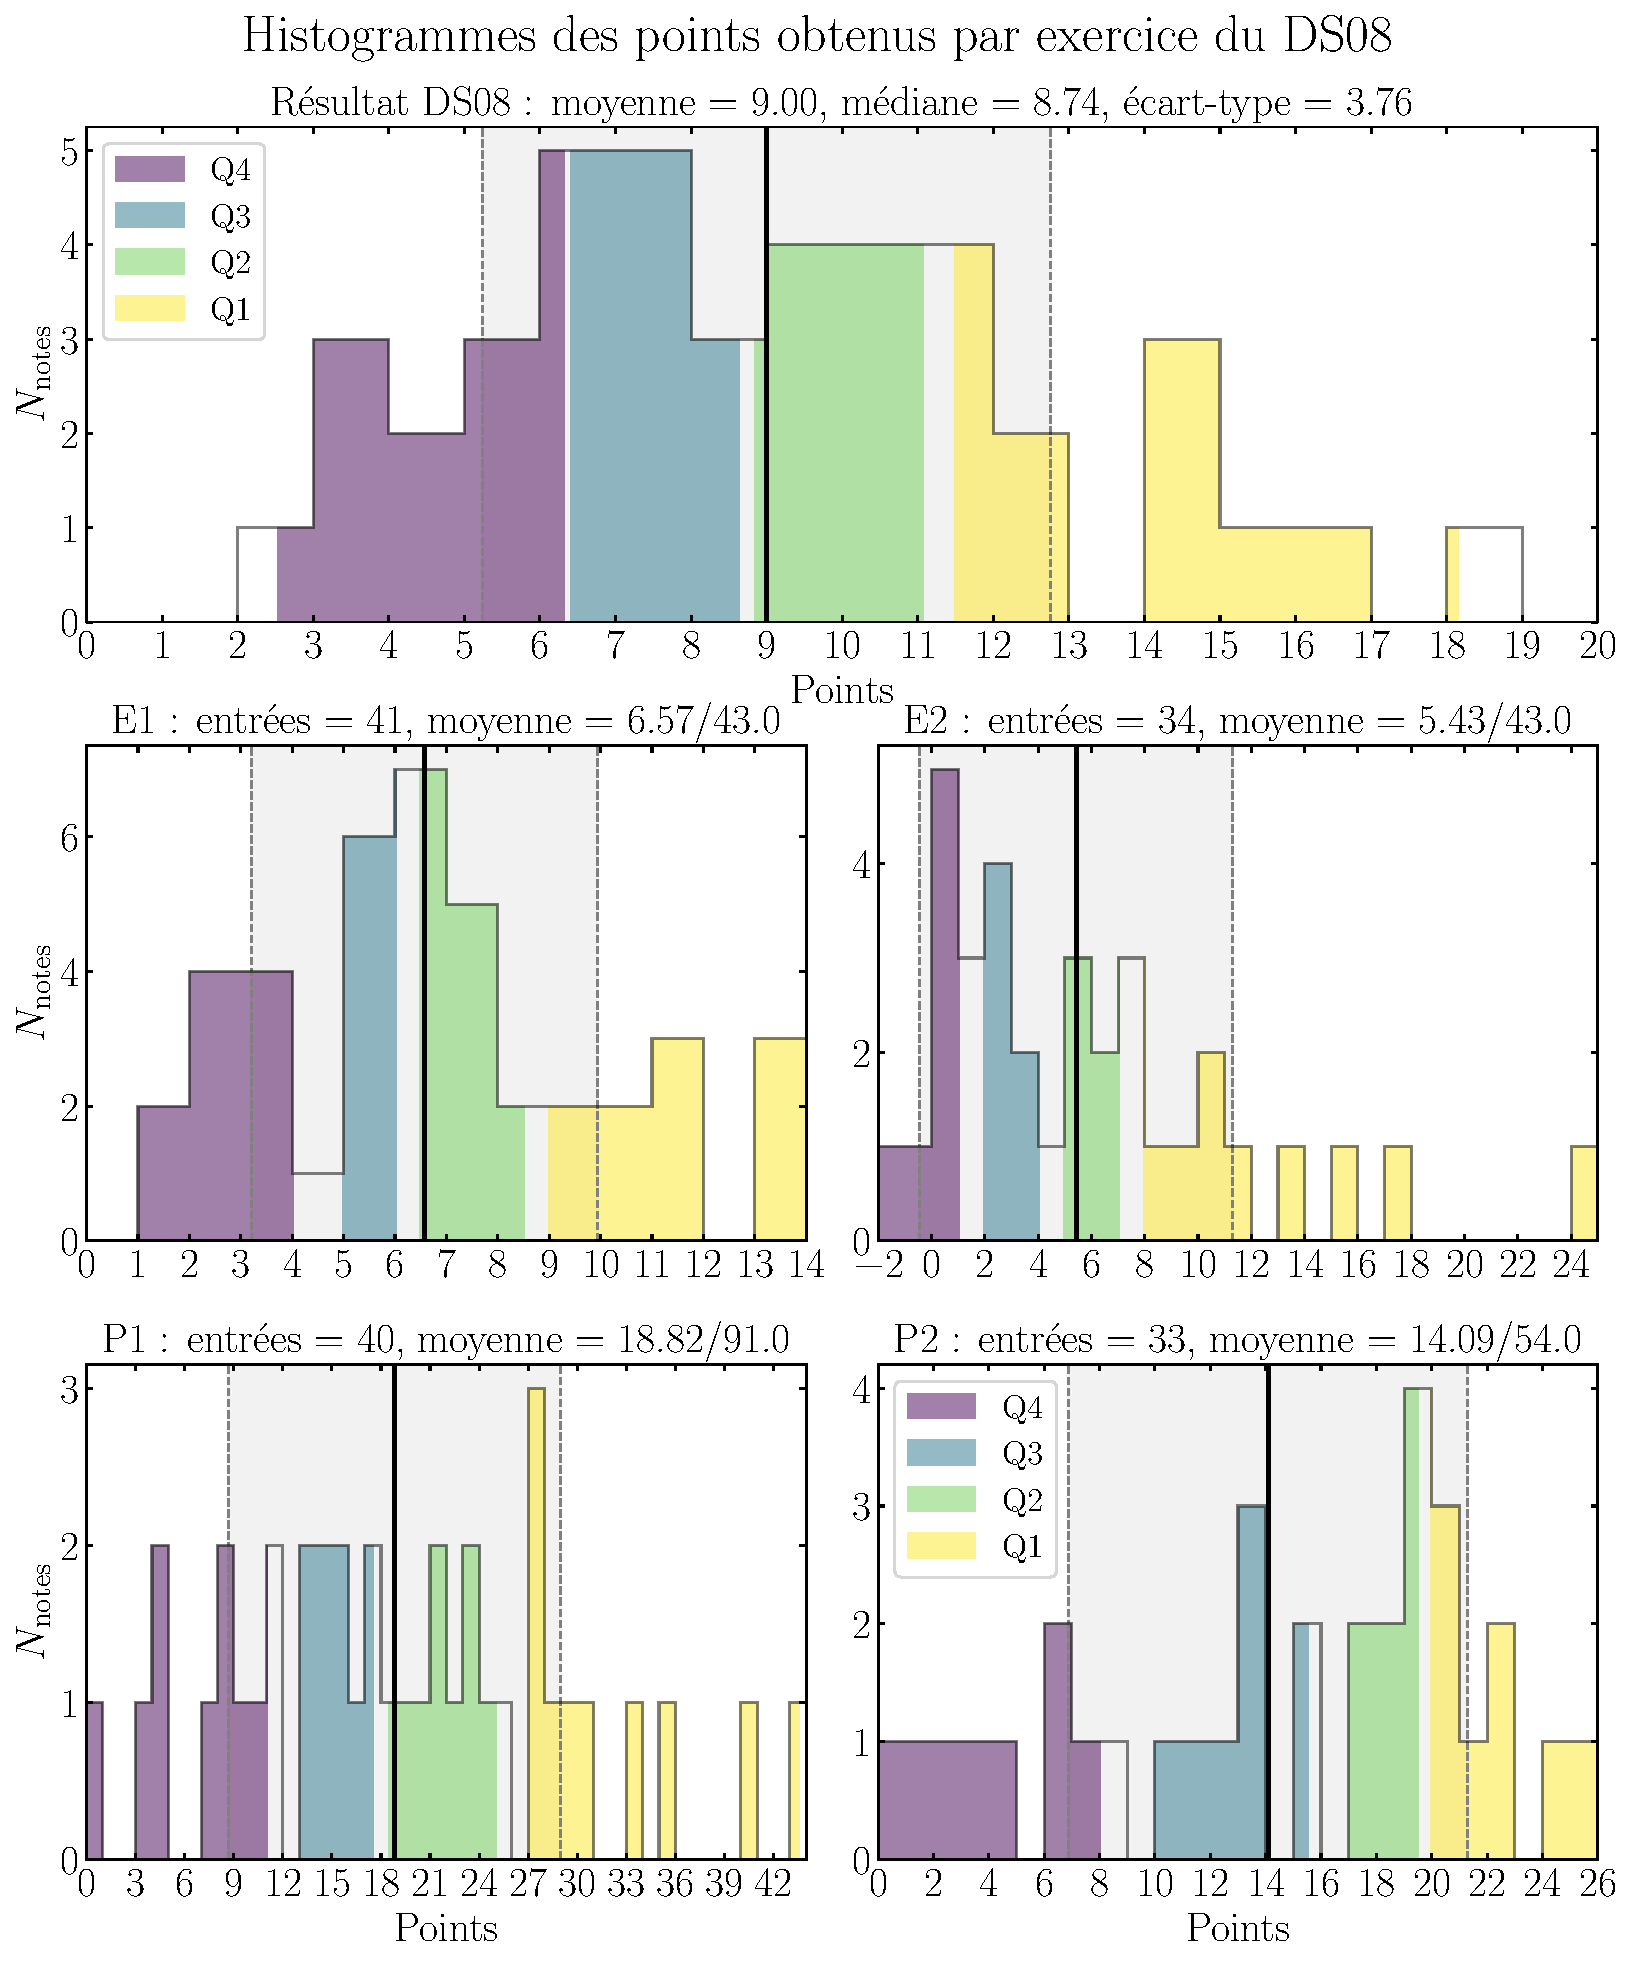
\includegraphics[width=1\linewidth]{DS01_hist_all}
\end{figure}

\setcounter{section}{0}
\section[32]"E"{Étude de quelques lentilles minces}

Très hétérogène. Il est clair de savoir qui travaille comme je le demande et qui
ne le fait pas. C'est décevant qu'une grande partie ne daigne pas travailler le
DS de l'année dernière.

En revanche, la quasi-totalité des schémas sont vraiment qualitatifs. Les rayons
incidents et émergents sont différenciés, les sens de comptage dessinés, les
règles primaires bien comprises. Bravo~!

Dans l'ensemble, revoir le concept de preuve. Il faut que vous soyez
convaicant-es.

\begin{enumerate}[label=\sqenumi]
	\item[n]{8}% Q1
	      \vspace{-22pt}
	      \begin{itemize}
		      \item Il faut indiquer les valeurs numériques pour les AN.
		      \item Ne donnez jamais le résultat littéral avec 0 ligne de calcul, il
		            \textbf{faut} détailler comment vous passez de la relation de
		            conjugaison à isoler la grandeur voulue.
		      \item Calcul $\neq$ mesure avec la règle.
		      \item Attention à bien prendre $\xul{\OA = \SI{-40}{cm}}$ (avec le
		            «~$-$~»)~!
		      \item Pensez bien à écrire complètement votre expression littérale avant
		            de l'encadrer/la calculer~:
		            \[
			            \frac{1}{\OAp} = \frac{1}{\OA} + \frac{1}{f'}
			            \qou
			            \OAp = \left[\frac{1}{\OA} + \frac{1}{f'}\right]^{-1}
		            \]
		            ne sont pas des réponses recevables.
	      \end{itemize}
	\item[n]{5}% Q2
	      Pas besoin de redémontrer le résultat littéral s'il est le même. Vous pouvez
	      juste le réécrire (en disant «~comme précédemment question 1~»), et indiquer
	      les nouvelles valeurs numériques pour l'AN.
	\item[n]{5}% Q3
	      \begin{itemize}
		      \item Lisez bien l'énoncé~: objet \textbf{virtuel} donc \textbf{derrière}
		            la lentille.

		      \item Il faut prolonger les rayons incidents pour montrer qu'ils se
		            croisent bien en B.
	      \end{itemize}
	\item[n]{3}% Q4
	      Bien~! Pas besoin de redémontrer.
	\item[n]{5}% Q5
	      Bien dans l'ensemble. C'est fâcheux, mais encore un certain nombre de
	      tentatives de preuves ne sont pas recevables. Trois schémas avec l'objet
	      avant, sur et après le foyer objet ne constitue pas une démonstration.
	      Il faudrait pour ça montrer que toutes les positions avant le foyer sont
	      similaires, et de même pour les positions après.
	\item[n]{4}% Q6
	      Bien. Beaucoup de tautologies qui ne démontrent rien («~l'image est
	      virtuelle car elle est avant la face d'entrée~»~: ok mais c'est la
	      définition d'une image virtuelle, ça n'est pas une preuve).
	\item[n]{2}% Q7
	      Bien.
\end{enumerate}

\section[35]"E"{Optique d'un périscope}
\begin{itemize}
	\item \textbf{Réponse sans justification = 0 !}
	\item Attention, beaucoup de problèmes de signes «~$-$~» dans les objets
	      réels~!
	\item \textbf{Vous ne pouvez pas trouver la réponse par élimination} dans ce
	      type de sujet. Vous pouvez le faire pour vous \textit{guider} et c'est
	      très malin, mais ça n'est pas une justification recevable scientifiquement.
\end{itemize}

\begin{enumerate}[label=\sqenumi]
	\item[n]{3}% Q1
	      Bien dans l'idée. \textbf{Attention}, on insiste bien dans l'énoncé que
	      $a$ est une \textbf{distance non algébrique}~!
	\item[n]{9}% Q2
	      \vspace{-22pt}
	      \begin{itemize}
		      \item Il faut \textbf{démontrer} que les points focaux doivent être
		            confondus.
		      \item \textbf{Ne confondez pas les points F$_1'$ ou F$_2$ avec les
			            distances focales $f_1'$ et $f_2$}~!! $f_1'$ et $f_2$ ne peuvent
		            être confondus, ce sont des distances.
		      \item Au risque de me répéter, \textbf{les lentilles divergentes n'ont
			            rien de spécial}. Cela n'a pas de sens de choisir $f_1' - f_2'$
		            «~parce que la lentille 2 est divergente~».
	      \end{itemize}
	\item[n]{9}% Q3
	      RAS, très compliqué.
	\item[n]{3}% Q4
	      Bien, récurrent problèmes de signe dans l'objet.
	\item[n]{3}% Q5
	      Idem.
	\item[n]{4}% Q6
	      Il faut justifier l'approximation des petits angles en \textbf{citant
		      les conditions de \textsc{Gauss}}. J'ai rajouté des points bonus pour
	      les schémas non demandés. C'est une bonne habitude à prendre. Bien sur
	      l'objet étendu.
	\item[n]{4}% Q7
	      Peu traité, mais quand même une justification qui fait sens.
\end{enumerate}

\setcounter{section}{0}
\section[51]"P"{Formation d'un arc-en-ciel}
Pour le décompte des points, à la fin le \textbf{total est multiplié par
	\num{1.5}}. C'est pour cela que la somme que vous comptez n'est pas la note
totale.
\begin{enumerate}[label=\sqenumi]
	\item[n]{3}% Q1
	      \vspace{-22pt}
	      \begin{itemize}
		      \item Pour les angles avec une valeur numérique, \textbf{utilisez les
			            radians} plutôt que les degrés~: on préfère écrire $\pi$ qu'un
		            «~sauvage~» \num{180}.
		      \item Attention aux angles orientés~! Vérifiez le signe avec le schéma.
	      \end{itemize}
	\item[n]{4}% Q2
	      \vspace{-22pt}
	      \begin{itemize}
		      \item \textbf{On écrit $\arcsin$ et pas $\sin^{-1}$ ou $\rm \asin$}~!
		      \item Attention aux notations~! Ici, $n\ind{eau} = n$.
		      \item Répondez bien à la question~!! On veut $i_2$, $i_3$ et $i_4$ en
		            fonction de $i_1$~!
		      \item ÉNORMÉMENT de lois de la réfraction à la place de la réflexion
		            (entre $i_3$ et $i_1$). C'est grave.
	      \end{itemize}
	\item[n]{2}% Q3
	      RAS.
	\item[n]{8}% Q4
	      Il faut faire attention à la variable de dérivation~! On ne vous donne pas
	      la dérivée de $\arcsin(\sin(x))$, ça n'aurait pas de sens. Bien dans l'idée
	      pour quelques copies.
	\item[n]{2}% Q5
	      Idem, $i_{1,\rm max}$ n'est pas $\sin(i_{1,\rm max})$.
	\item[n]{2}% Q6
	      Utilisez la figure.
	\item[n]{1}% Q7
	      RAS.
	\item[n]{8}% Q8
	      Question très intéressante, je vous invite à bien lire le corriger pour
	      vraiment comprendre l'origine des arcs-en-ciel. Un schéma est nécessaire, et
	      il faut faire attention à la valeur absolue de la déviation.
	\item[n]{4}% Q9
	      Quelques bonnes réponses~!
\end{enumerate}

\section[75]"P"{Module photographique d'un smartphone}
\begin{enumerate}[label=\sqenumi]
	\item[n]{5} % Q1
	      La diagonale d'un \textbf{rectangle} ne forme pas un angle de
	      $\ang{45}$~! Et un capteur de taille $\num{4000}a\times \num{3000}a$ ne
	      saurait être un carré~! TB pour les schémas réalistes cependant.
	\item[n]{4} % Q2
	      Dire «~Voir annexe~». La construction des rayons quelconques n'est pas
	      maîtrisée, c'est dommage.
	\item[n]{6} % Q3
	      Jamais faite.
	\item[n]{3} % Q4
	      RAS.
	\item[n]{10} % Q5
	      Dire «~Voir annexe~». Trop de confusions entre le rayon et l'angle
	      d'incidence. Attention, dioptre verre-air $\neq $ dioptre air-verre~!
	      Attention à la position du point I.
	\item[n]{5} % Q6
	      Jamais fait. C'était \textbf{bizarrement} presque équivalent au dernier
	      exercice du soutien de la veille. Tiens tiens…
	\item{}[\fbox{7-13}] % Q7
	      RAS.
	      % \item[n]{2} % Q8
	      %   RAS.
	      % \item[n]{6} % Q9
	      % \item[n]{10} % Q10
	      % \item[n]{5} % Q11
	      % \item[n]{6} % Q12
	      % \item[n]{8} % Q13
\end{enumerate}

\end{document}
